\documentclass{beamer}
\usepackage{hyperref}
\usepackage{url}
\usepackage{natbib}
\usepackage{xcolor}
\usepackage{graphicx}
%\usepackage{enumitem}  
\usepackage{calc}  
\usepackage{amsmath}
\usepackage{amssymb}
\usepackage{amsthm}
\usepackage{thmtools}

\usepackage{xspace}

% \usepackage{tikz}
%\usetheme{vub} 
% \usetheme{Copenhagen}
\usetheme{Madrid}
\usecolortheme{rose}
%  \usetheme[coloredtitles]{vub}
% \usetheme[showsection]{vub}
\title{Visual Step-By-Step Explanations of Constraint Satisfaction Problems}
\subtitle{ZebraTutor - Explaining logic grid puzzles}
\author{Emilio Gamba\textsuperscript{1}, Bart Bogaerts\textsuperscript{2}, Tias Guns\textsuperscript{1}\\\tiny{\textsuperscript{1}data-lab, Vrije Universiteit Brussel}\\
\tiny{\textsuperscript{2}AI lab, Vrije Universiteit Brussel}\\
\tiny{\{firstname.lastname\}@vub.be}}
\date{}

\newcommand\m[1]{\ensuremath{#1}\xspace}
\newcommand\allconstraints{\m{T_P}}

\newcommand{\phantomgraphics}[2][]{%
  \leavevmode\phantom{\includegraphics[#1]{#2}}%
}


\begin{document}

% \begin{frame}{\small{Explainable Artificial Intelligence (XAI)}}
%     \maketitle
% \tiny{\textsuperscript{1}data-lab, Vrije Universiteit Brussel}\\
% \tiny{\textsuperscript{2}AI lab, Vrije Universiteit Brussel}\\
% \tiny{\{firstname.lastname\}@vub.be}
% \end{frame}
% Automatic titlepage with VUB logo.
\frame{\maketitle

}
%a
\begin{frame}{\small{Explainable Artificial Intelligence (XAI)}}
    \framesubtitle{Motivation}
    \textbf{Curse of performance}
    \begin{itemize}
        \item Black-box prediction systems (e.g. deep neural networks)
        \item Efficient complex reasoning systems with millions of parameters
    \end{itemize}

    \begin{figure}[]
        \centering
        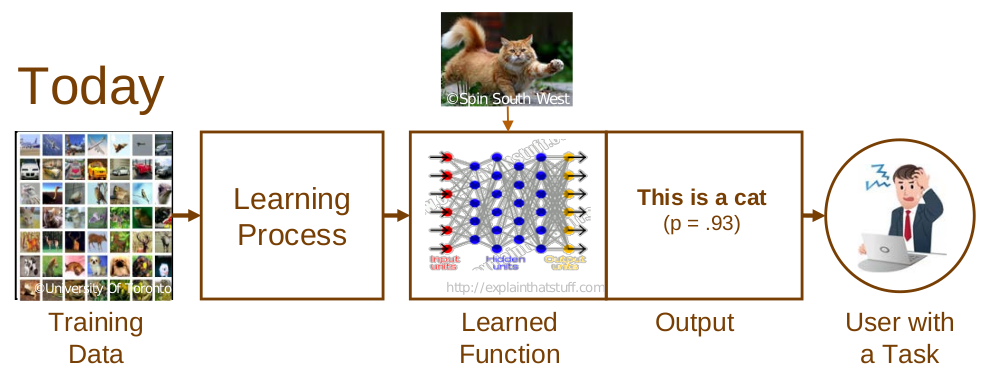
\includegraphics[width=0.8\textwidth]{figures/cat}
        {\small \caption{Deep neural network - image classifier \textsuperscript{\cite{gunning2017explainable}}}}
        \label{catdog}
    \end{figure}

\end{frame}

\begin{frame}{\small{Explainable Artificial Intelligence (XAI)}}
    \framesubtitle{Motivation}
    \begin{block}{Human-interpretability}
        \emph{Users should be able to \textbf{see} but also \textbf{study} and \textbf{understand} how inputs are mathematically mapped to outputs.} \textsuperscript{\cite{doran2017does}}
    \end{block}
    \vfill
    \textbf{The A.R.T of Responsible AI \textsuperscript{\cite{adadi2018peeking}}}
    \begin{itemize}
        \item \textbf{\underline{A}ccountability} \textit{need to explain and justify actions to user}
        \item \textbf{\underline{R}esponsibility} \textit{role of answering for one's decisions and identify errors or unexpected results}
        \item \textbf{\underline{T}ransparency} \textit{need to describe, inspect reproduce AI thought process}
    \end{itemize}

\end{frame}

\begin{frame}{\small{Explainable Artificial Intelligence (XAI)}}
    \framesubtitle{Definition}
    \vfill

    \begin{center}
        \emph{``XAI is an explanatory agent revealing underlying \textbf{causes} to its or another agent’s decision making''} \textsuperscript{\citep{miller2019explanation}}
    \end{center}
    \begin{flushright}
        --- Miller, 2019
    \end{flushright}
    \vfill

\end{frame}

\begin{frame}{\small{Explaining Constraint Satisfaction Problems}}
    \framesubtitle{Goal : Explainable agency}

    Given \emph{objectives} and \emph{background knowledge} relevant to objectives:
    \begin{itemize}
        \item \small{Produce \emph{records of decision} taken during plan generation}
        \item \small{Produce summary of agent's \emph{mental effort}}
        \item \small{Produce \emph{understandable explanations} about specific choices and reasons for them}
    \end{itemize}
    \vspace*{1em}
    \begin{figure}[]
        \centering
        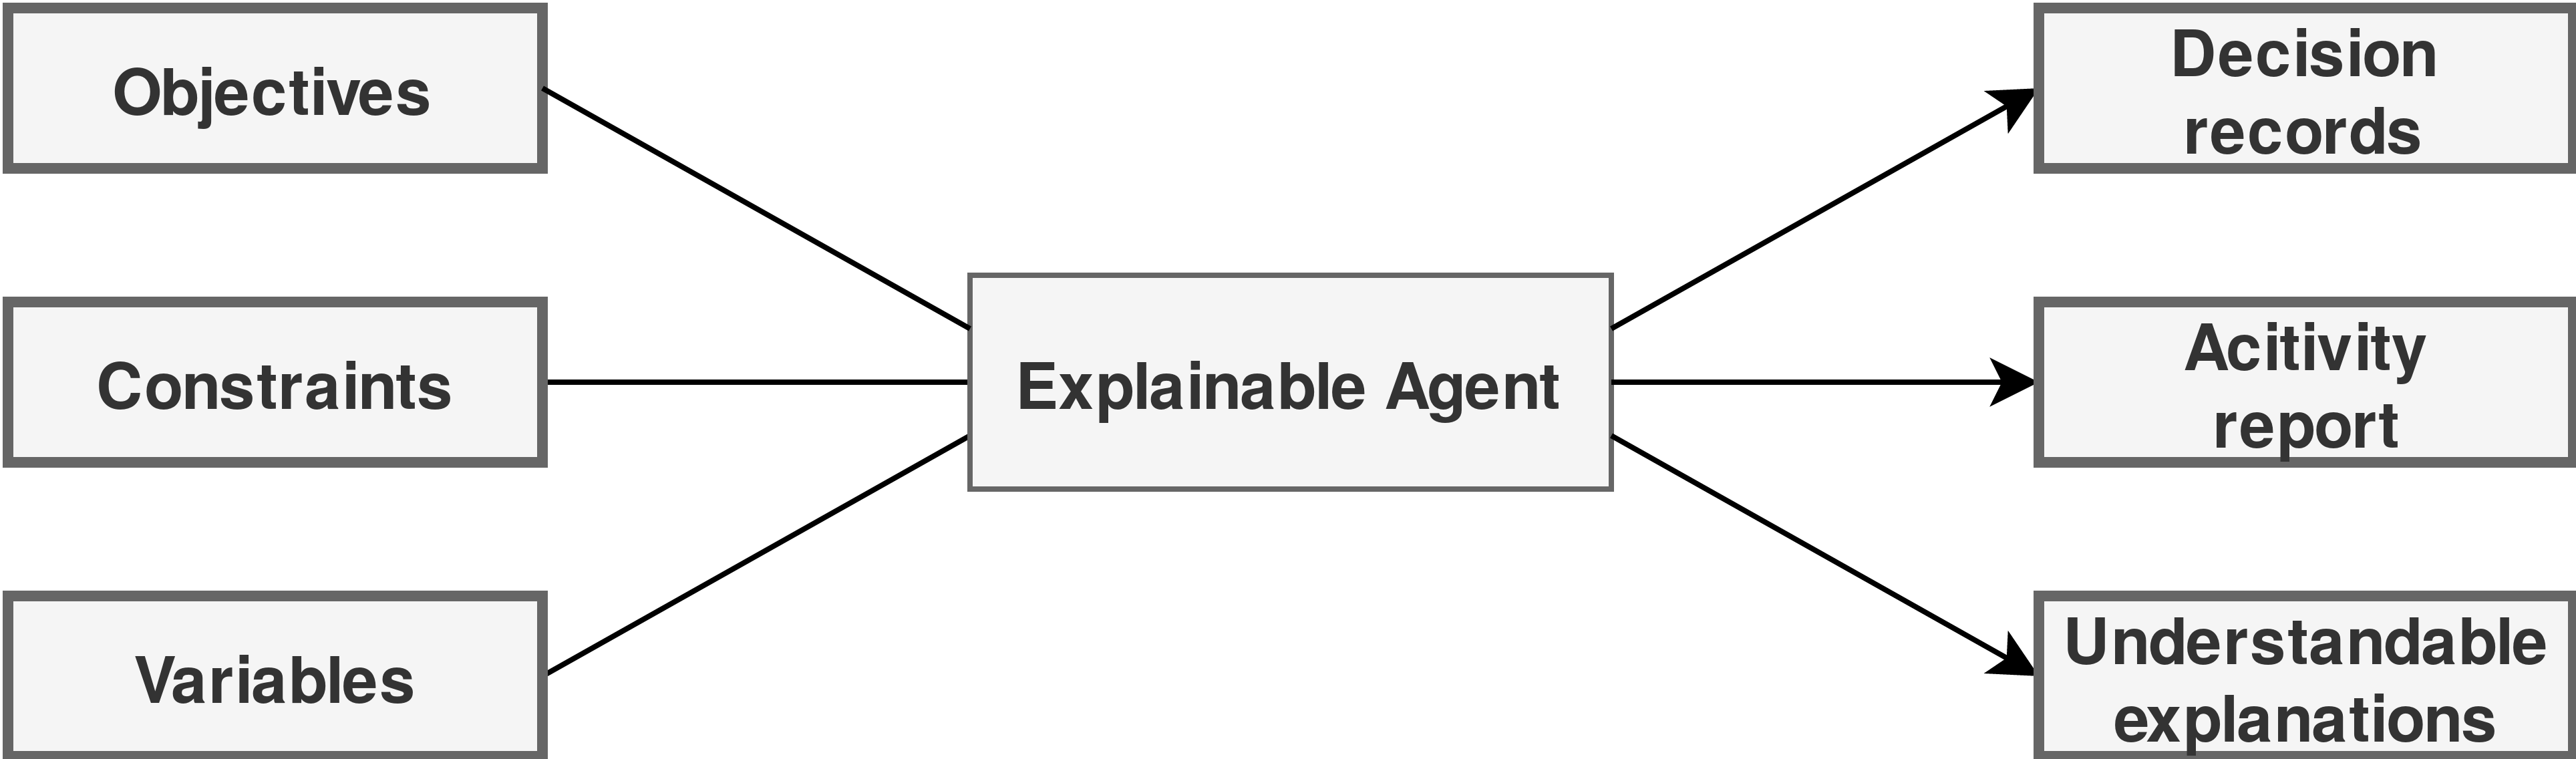
\includegraphics[width=0.8\textwidth]{figures/explainable_agency2}
    \end{figure}


\end{frame}


\begin{frame}{\small{Explaining Constraint Satisfaction Problems}}
    \framesubtitle{ZebraTutor : an \emph{explainable} agent }

    \only<1>{
        \begin{block}{Problem statement}
            Given the natural language problem statement and set of clues (entities, constraints)
        \end{block}
        \vfill
        \begin{figure}[]
            \centering
            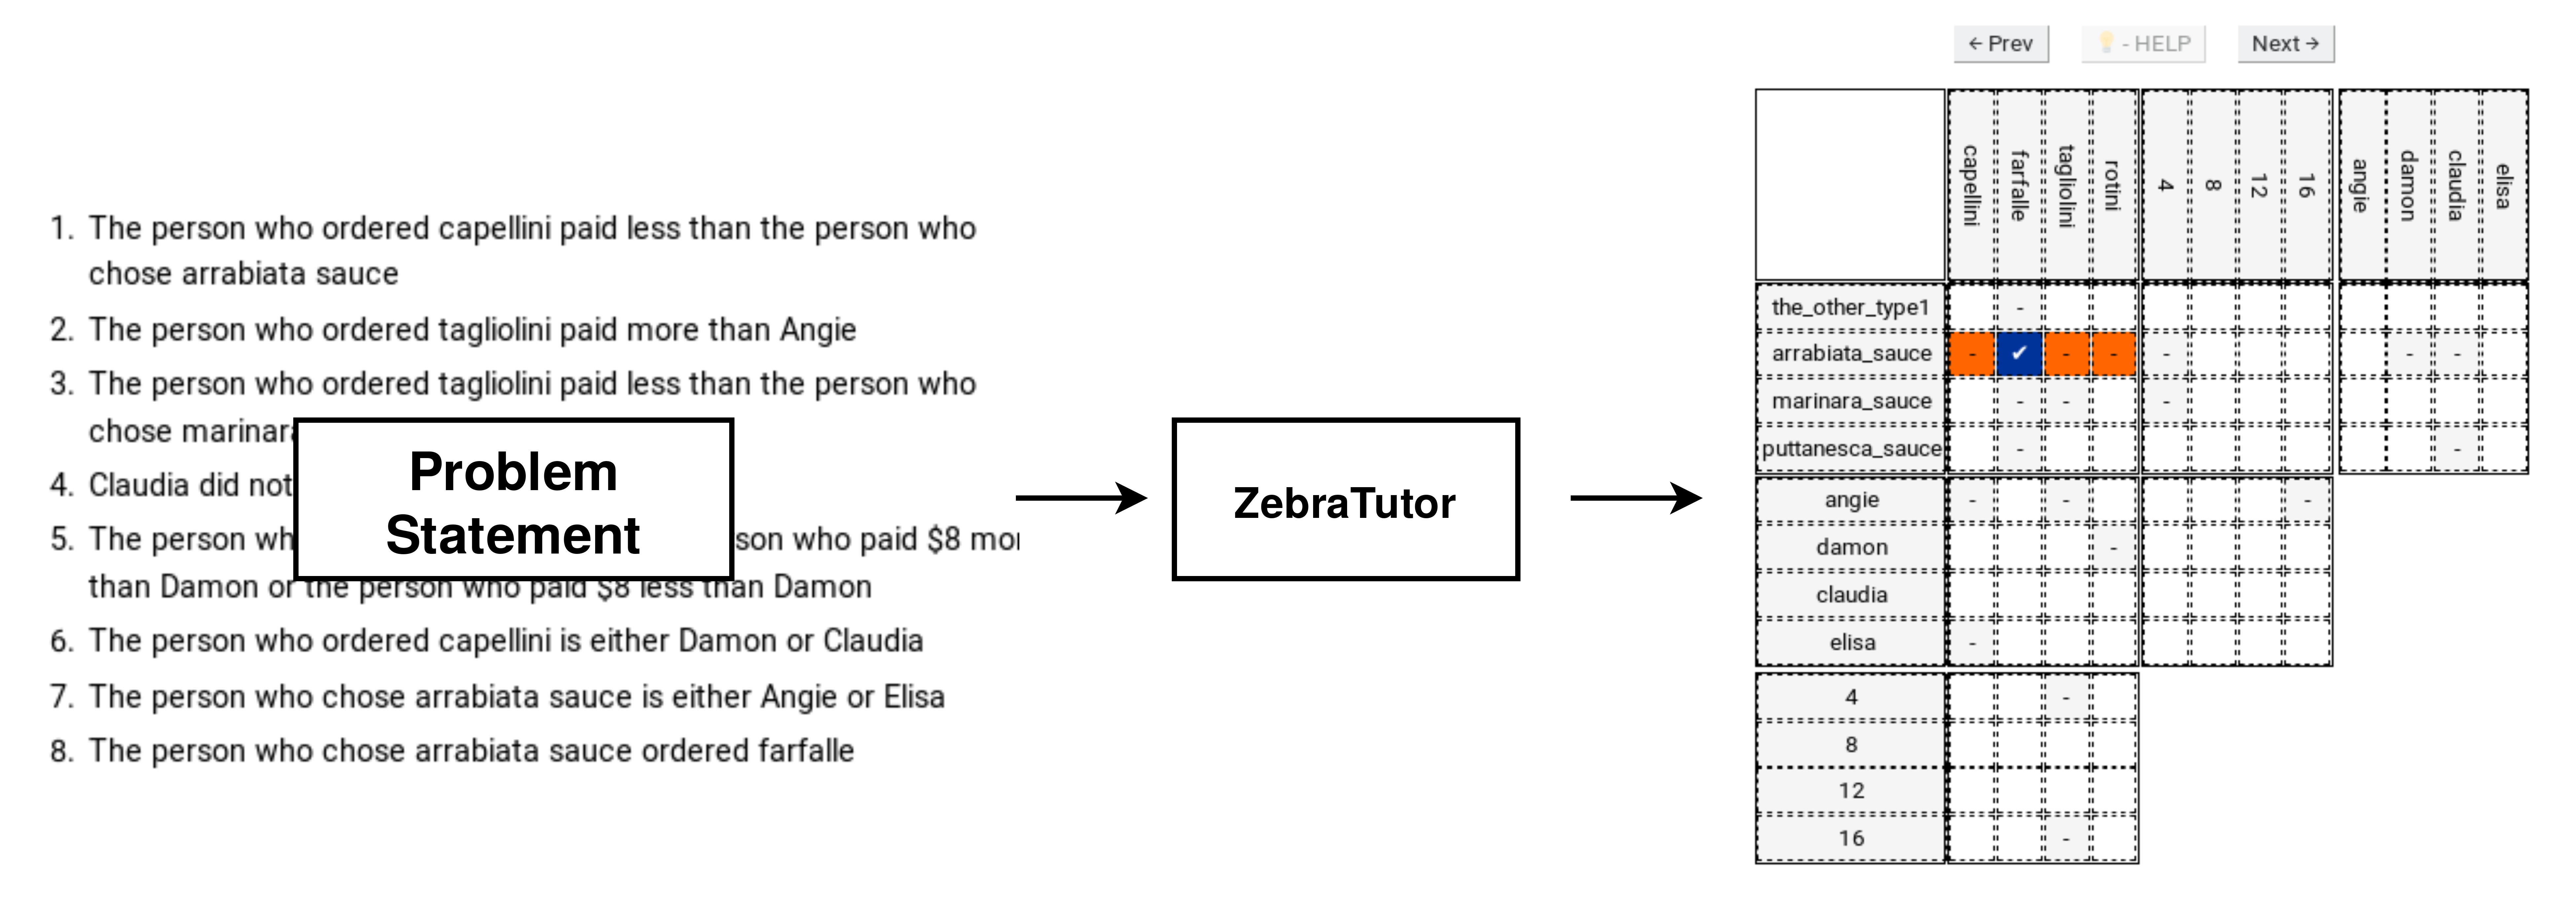
\includegraphics[width=\textwidth]{figures/puzzle_pipeline_4}
        \end{figure}
    }
    \pause
    \only<2>{
        \begin{block}{Problem statement}
            Given the natural language problem statement and set of clues (entities, constraints):
            \begin{itemize}
                \item Produce the \emph{explanation sequence} to solve the puzzle
                      \phantom{\parbox{\linewidth}{\item Produce the cost (mental effort) associated to each step}}
                      \phantom{\parbox{\linewidth}{\item Produce the \emph{cognitively-easiest explanation} for each step in the explanation sequence}}
            \end{itemize}
        \end{block}
        \begin{figure}[]
            \centering
            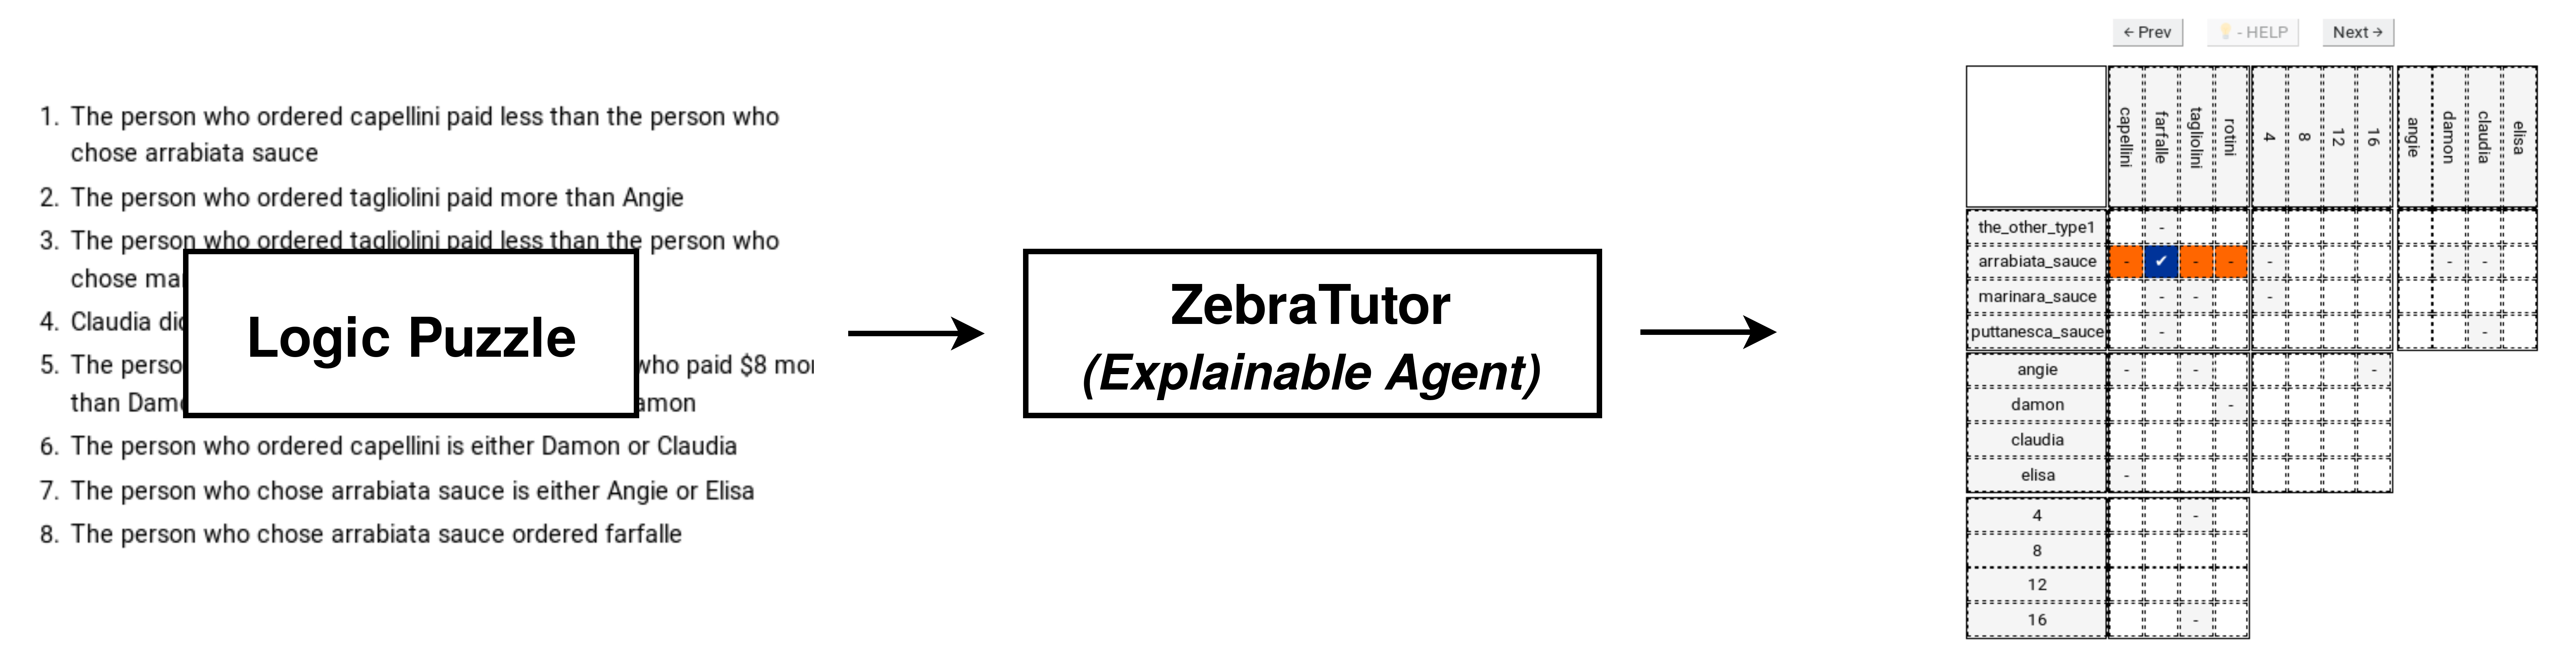
\includegraphics[width=0.8\textwidth]{figures/puzzle_pipeline}
        \end{figure}
    }

    \pause
    \only<3>{
        \begin{block}{Problem statement}
            Given the natural language problem statement and set of clues (entities, constraints):
            \begin{itemize}
                \item Produce the \emph{explanation sequence} to solve the puzzle
                \item Produce the cost (mental effort) associated to each step
                      \phantom{\parbox{\linewidth}{\item Produce the \emph{cognitively-easiest explanation} for each step in the explanation sequence}}
            \end{itemize}
        \end{block}
        \begin{figure}[]
            \centering
            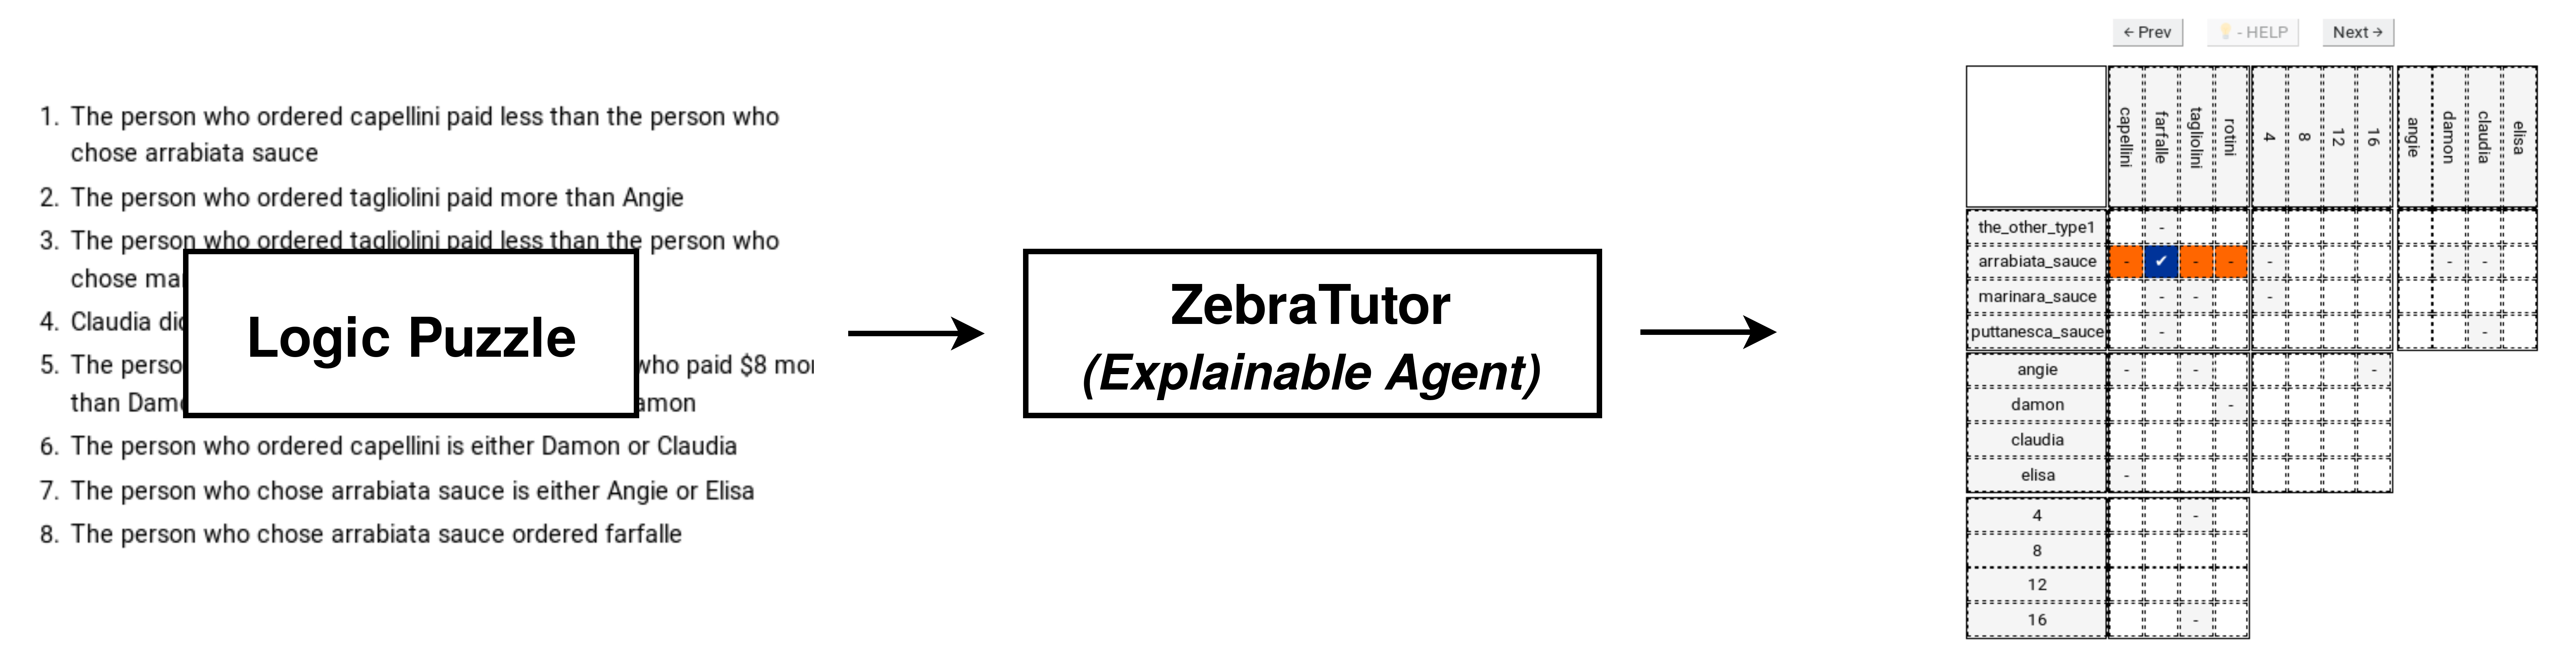
\includegraphics[width=0.8\textwidth]{figures/puzzle_pipeline}
        \end{figure}
    }

    \pause
    \only<4>{
        \begin{block}{Problem statement}
            Given the natural language problem statement and set of clues (entities, constraints):
            \begin{itemize}
                \item Produce the \emph{explanation sequence} to solve the puzzle
                \item Produce the cost (mental effort) associated to each step
                \item Produce the \emph{cognitively-easiest explanation} for each step in the explanation sequence
            \end{itemize}
        \end{block}
        \begin{figure}[]
            \centering
            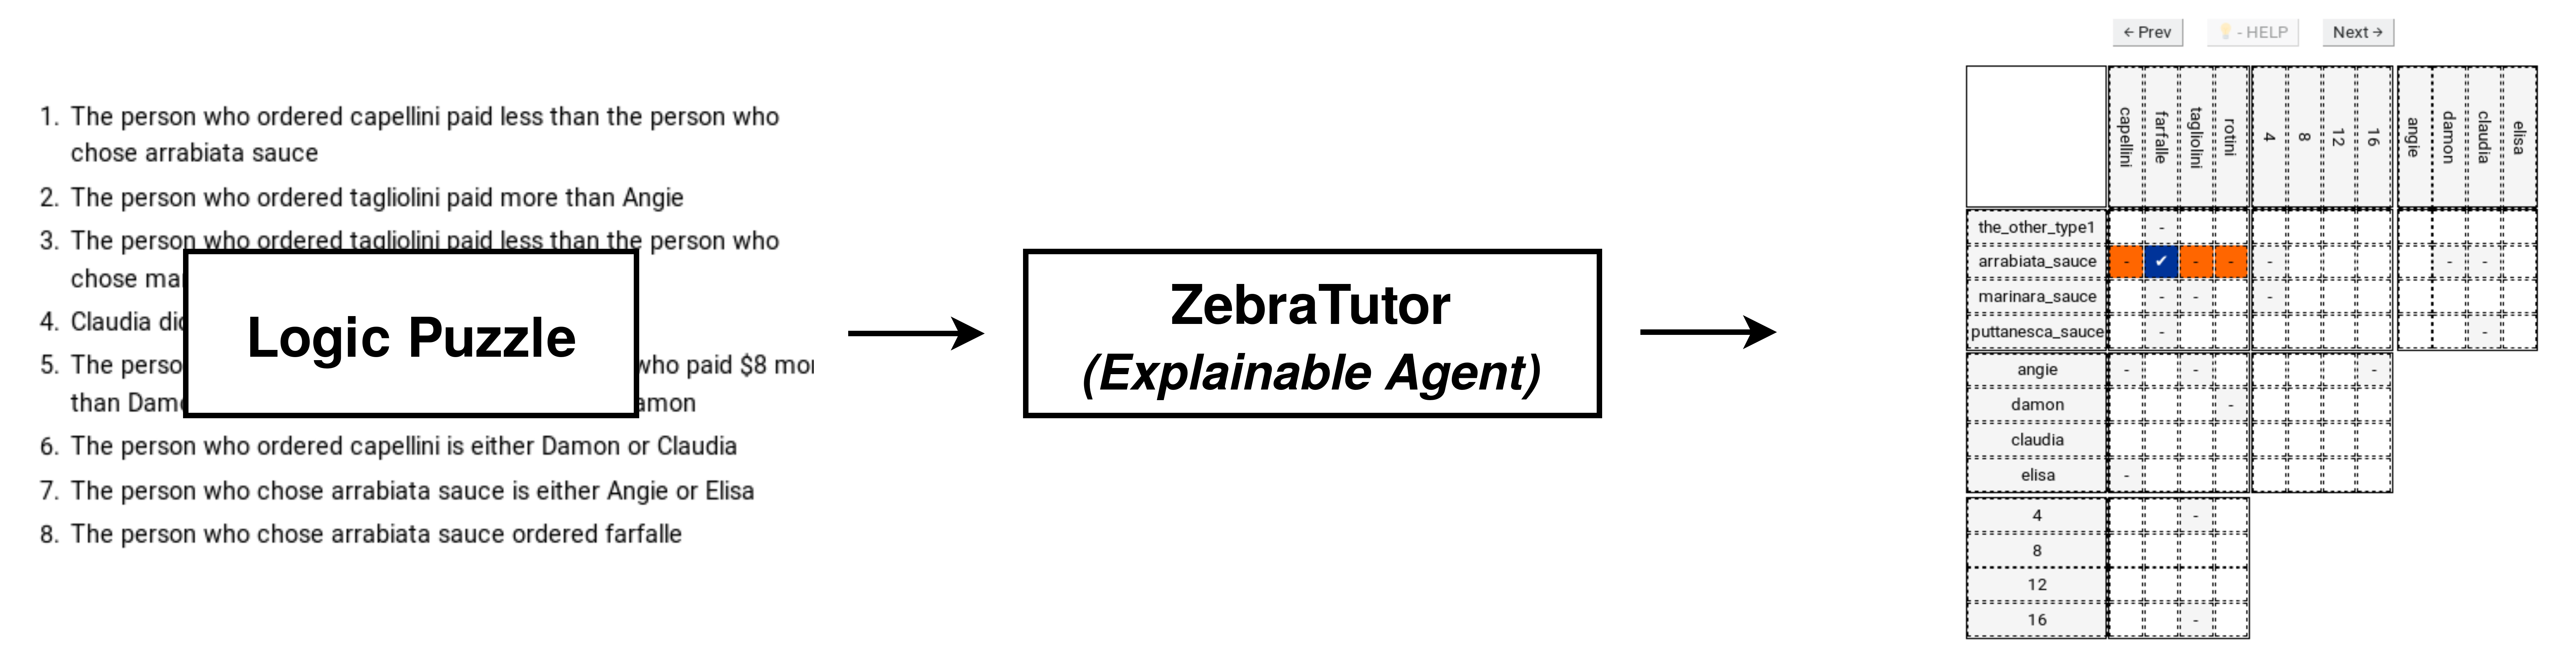
\includegraphics[width=0.8\textwidth]{figures/puzzle_pipeline}
        \end{figure}
    }

    % \vfill


\end{frame}

\begin{frame}{\small{Explaining Constraint Satisfaction Problems}}
    \framesubtitle{ZebraTutor : an \emph{explainable} agent }
    % \vspace{1cm}
    % \only<1>{
    %     \begin{block}{Problem statement}
    %         Given the natural language problem statement and set of clues (entities, constraints):
    %         \begin{itemize}
    %             \item Produce the \emph{explanation sequence} to solve the puzzle
    %             \item Produce the cost (mental effort) associated to each step
    %             \item Produce the \emph{cognitively-easiest explanation} for each step in the explanation sequence
    %         \end{itemize}
    %     \end{block}
    %     \phantomgraphics[width=\textwidth]{figures/step_1}%
    % }
    % \only<8>{

    % }
    % \vfill
    % \pause
    \only<1-8>{
        \begin{block}{\textcolor{lightgray}{Problem statement}}
            \textcolor{lightgray}{
                Given the natural language problem statement and set of clues (entities, constraints):}
            \begin{itemize}
                \item \textcolor{lightgray}{Produce the \textcolor{black}{\emph{explanation sequence}} to solve the puzzle}
                \item \textcolor{lightgray}{Produce the cost (\textcolor{black}{mental effort}) \textcolor{black}{associated to each step}}
                \item \textcolor{lightgray}{Produce the \textcolor{black}{\emph{cognitively-easiest explanation}} for each step in the explanation sequence}
            \end{itemize}
        \end{block}
    }
    \only<1>{\begin{figure}[]
            \centering
            
\includegraphics[width=\textwidth]{figures/step_1}
        \end{figure}}
    \pause
    \only<2>{\begin{figure}[]
            \centering
            
\includegraphics[width=\textwidth]{figures/step_2}
        \end{figure}}
    \pause
    \only<3>{\begin{figure}[]
            \centering
            
\includegraphics[width=\textwidth]{figures/step_3}
        \end{figure}}
    \pause
    \only<4>{\begin{figure}[]
            \centering
            
\includegraphics[width=\textwidth]{figures/step_4}
        \end{figure}}
    \pause
    \only<5>{\begin{figure}[]
            \centering
            
\includegraphics[width=\textwidth]{figures/step_5}
        \end{figure}}
    \pause
    \only<6>{\begin{figure}[]
            \centering
            
\includegraphics[width=\textwidth]{figures/step_6}
        \end{figure}}
    \pause
    \only<7>{\begin{figure}[]
            \centering
            
\includegraphics[width=\textwidth]{figures/step_7}
        \end{figure}}
    \pause
    \only<8>{

        \begin{figure}[]
            \centering
            
\includegraphics[width=\textwidth]{figures/step_8}
        \end{figure}}

\end{frame}

\begin{frame}{\small{Explaining Constraint Satisfaction Problems}}
    \framesubtitle{ZebraTutor : background}
    % \vspace{1.5cm}
    \begin{block}{Typed Entity} \textit{Elisa} \texttt{[Person]}, \textit{farfalle} \texttt{[Pasta]}\end{block}
    \vspace{0.5em}
    \begin{block}{Literal} relation between entities $chose(Elisa, farfalle)$\end{block}
    \vspace{0.5em}
    \begin{block}{Clue}A clue is a first-order logic theory $\allconstraints$
    \begin{center}
        ``\emph{The person who chose arrabiata sauce ordered farfalle}''\\
        \vspace{0.5em}
        $\exists$ p \texttt{[Person])} : chose(p, arrabiata) $\wedge$ ordered(p, farfalle)
    \end{center}
\end{block}
    
\end{frame}

\begin{frame}{\small{Explaining Constraint Satisfaction Problems}}
    \framesubtitle{ZebraTutor : csp problem definition}
    \vfill
    \textbf{Goal} Find relations between each two types s.t.:
    {\small
    \begin{itemize}
        \item Each clue is respected
        \item \textbf{Bijectivity} Entity of 1 type is matched exactly with 1 entity of the second type (reverse holds)
        \item \textbf{Transitivity} Relations are logically linked:\\
              ``If Angie chose arrabiata sauce, and arrabiata sauce is paired with farfalle, then Angie must have eaten farfalle''
    \end{itemize}
    }

\end{frame}


\begin{frame}{\small{Explaining Constraint Satisfaction Problems}}
    \framesubtitle{ZebraTutor : background}
    % \vspace{1.5cm}
    \begin{block}{(Partial) Interpretation}
        Finite set of literals of the form $P(\overline{d})$ or $\neg P(\overline{d})$
        \begin{description}
            \item[$P$] {\small where  is a relation symbol typed $T_1 \times ... \times T_n$}
            \item[$\overline{d}$] {\small where  is tuple of domain elements, $d_i$ is of type $T_i$}
            \item[$I_1$] $\{chose(Elisa, farfalle), \neg chose(Angie, farfalle) \}$
        \end{description}
    \end{block}
    \begin{block}{Full Interpretation $I$}
        I contains $P(\overline{d})$ or $\neg P(\overline{d})$ for each well-typed atom $P(\overline{d})$
    \end{block}

    \begin{block}{$I_2 \geq_p I_1$}
        Interpretation $I_2$ is more precise than $I_1$  iff $I_2$ contains at least all the literals of $I_1$  
   \end{block}
\end{frame}

\begin{frame}{\small{Explaining Constraint Satisfaction Problems}}
    \framesubtitle{ZebraTutor : background}
    % \vspace{1.5cm}

    % \begin{block}{Full Interpretation $I$}
    %     I contains $P(\overline{d})$ or $\neg P(\overline{d})$ for each well-typed atom $P(\overline{d})$
    % \end{block}

    \begin{block}{Maximal consequence max($I$, $\allconstraints$)}
        The \textit{maximal consequence  of a theory $\allconstraints$}, and \textit{partial interpretation I},  $J$ is the precision-maximal partial interpretation J s.t. $I \wedge \allconstraints \models J$
    \end{block}

    \begin{block}{Sequence of incremental partial interpretations}
        A \textit{sequence of incremental partial interpretations} of a theory $\allconstraints$ with initial partial interpretation $I_0$ is a sequence $\langle I_0, I_1, \ldots, I_n  = max(I_0,\allconstraints)\rangle$ where $\forall i>0, I_{i-1} \leq_p I_{i}$ (i.e., the sequence is precision-increasing).
    \end{block}
    
\end{frame}

% \begin{frame}{\small{Explaining Constraint Satisfaction Problems}}
%     \framesubtitle{ZebraTutor : background (2)}

%     A sequence $\langle I_0, I_1, ..., I_n = max(I, \allconstraints)\rangle$ where 

% \end{frame}






    % \begin{center}
    %     \emph{``Given a set of theories, find an interpretation I that satisfies all the constraints''}
    % \end{center}


\bibliographystyle{abbrv}
\begin{frame}
    \frametitle{References}
    \vspace{2em}
    \bibliography{references}
\end{frame}

\end{document}